\chapter{Budowa modeli}

\section{Jednowarstwowa architektura LSTM}
\label{section:one_lstm}

Pierwszy model bazuje na zaproponowanej przez organizatorów konkursu jednowarstwowej architekturze sieci rekurencyjnej z komórkami LSTM. Zastosowanie tej budowy modelu zapewnia zdolność do uczenia się długoterminowych zależności przy jednoczesnym unikaniu długotrwałego problemu uzależnienia. 

Przygotowawczym etapem modelu jest przedstawienie wymagań dla danych, które mogą być przetwarzane w warstwie wejściowej (ang. \textit{Input Layer}). Każdy przykład jest przetworzony zgodnie z opisem w rozdziale \ref{chapter:przetwarzanie_danych}. Jednym z ostatnich etapów przetwarzania jest wyrównanie wszystkich przykładów do równej długości w tym przypadku 200, zgodnie z rysunkiem \ref{rys:lstm_one_graph} przedstawiającym budowę jednowarstwowej architektury LSTM.

\begin{figure}[t]
\centering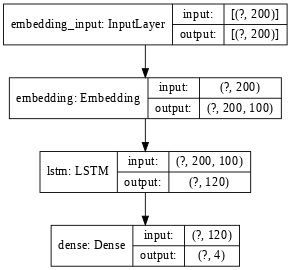
\includegraphics[width=6cm]{figures/reports/lstm_one_graph.png}
\fcmfcaption{Graf przedstawiający budowę jednowarstwowej architektury LSTM.}\label{rys:lstm_one_graph}
\end{figure}

Kolejną warstwą jest zamiana reprezentacji słowa na gęstą reprezentację wektorową opisaną w sekcji \ref{section:words_embeddings}. Do uzyskania tej reprezentacji użyto gotowe macierze udostępnione przez autorów metody na stronie internetowej\footnote{\url{https://nlp.stanford.edu/projects/glove/}}. Do wyboru były macierze przygotowane na różnych zbiorach danych oraz o różnych szerokościach wektorów. Testy przeprowadzono z użyciem zagłębień słów wytrenowanych na zbiorze danych pochodzących z Wikipedii oraz z archiwum danych tekstowych Gigaword 5 (ang. \textit{English Gigaword Fifth Edition}). Wybór szerokości wektorów podyktowany był złożonością modelu i czasem nauki, z pośród zbioru 50, 100, 200, 300 zdecydowano się na szerokość 100. Podsumowując złożoność tego etapu zawiera on prawie 2 miliony wewnętrznych parametrów (wag), które są zamrożone na czas uczenia. Rysunek \ref{rys:lstm_one_table} przedstawia szczegóły budowy jednowarstwowej architektury LSTM, wraz z tą warstwą o nazwie \textit{Embedding}.

\begin{figure}[t]
\centering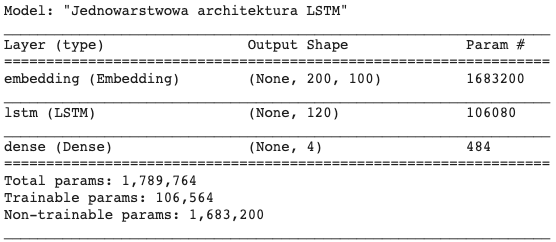
\includegraphics[width=10cm]{figures/reports/lstm_one_table.png}
\fcmfcaption{Tabela przedstawiająca szczegóły budowy jednowarstwowej architektury LSTM.}\label{rys:lstm_one_table}
\end{figure}

Do stworzenia kolejnej warstwy użyto gotową reprezentację LSTM z pakietu tensorflow o nazwie \texttt{keras.layers.LSTM}, która udostępnia możliwość definiowania konkretnych szczegółów implementacyjnych. W warstwie tej użyto domyślną funkcję aktywacji jakim jest tangens hiperboliczny. Po obserwacji krzywej uczenia reprezentującej dokładność oraz wartość funkcji straty zauważono zjawisko przeuczenia. Dokładność dla zbioru uczącego rosła wraz z malejącą dokładnością dla zbioru walidacyjnego. Z tego powodu zdecydowano się na użycie metody przerywania (ang. \textit{dropout}), zdefiniowanej w tej warstwie. Pomogło to zmniejszyć wpływ zjawiska przeuczania się modelu.

Ostatnim etapem jest wybór odpowiedniej etykiety emocji za pomocą warstwy gęstej. Wyjście z poprzedniej warstwy nazywane stanem ukrytym (ang. \textit{hidden state}) o szerokości 120 jest gęsto połączone z 4 neuronami decydującymi odpowiednio o każdej z kolejnych etykiet emocji. Jako funkcję aktywacji tej warstwy, zgodnie z sugestią organizatorów konkursu użyto funkcję sigmoidalną. Zauważona jednak została niekompatybilność tej funkcji z konkretnym zastosowaniem dla klasyfikacji wieloklasowej co zostało poprawione w kolejno zaprezentowanych modelach.  

Końcowym elementem budowy tego modelu jest wybór algorytmu optymalizacyjnego. Wybrano algorytm RMSprop \cite{ruder2016overview} (ang. \textit{Root Mean Square Propagation}), który dobrze radzi sobie z wygasającymi wskaźnikami uczenia oraz przeciwdziała obliczeniowym problemom numerycznym. Jako funkcję straty użyto \textit{Categorical Cross-Entropy loss}, która bardzo dobrze radzi sobie w problemach klasyfikacji wielu klas.

\section{Głęboka architektura LSTM}
\label{section:deep_lstm}

Głęboka architektura LSTM jest rozszerzeniem architektury jednowarstwowej opisanej w punkcie \ref{section:one_lstm}. Głównym celem było porównanie złożoności architektury płytkiej i głębokiej oraz wpływ rozszerzenia modelu o kolejne warstwy na wynik. Modyfikacje polegały przede wszystkim na dodaniu kolejnych warstw oraz lekkie modyfikacje parametrów oraz funkcji wewnątrz modelu. Pierwsze dwie warstwy, wejściowa (\textit{Input Layer}) oraz mapująca słowa na gęstą reprezentację wektorową (\textit{Embedding}) zostały bez zmian.

Do rozszerzenia jednowarstwowej części sieci rekurencyjnej zamiast zwykłych komórek LSTM użyto dwukierunkowych komórek LSTM. Z założenia rozszerzenie to powinno poprawić wydajność modelu przy problemach z klasyfikacją sekwencji \cite{ding2018densely}. W tym przypadku można było użyć tego rozszerzenia ponieważ od razu są dostępne wszystkie sekwencje czasowe sekwencji wejściowej. W tym momencie dwukierunkowe komórki LSTM łączą dwie ukryte warstwy o przeciwnych kierunkach. Dzięki tej formie uczenia warstwa wyjściowa może jednocześnie uzyskiwać informacje z przeszłych jak i przyszłych stanów, co nie było możliwe przy użyciu podstawowych komórek LSTM. Zabieg ten pomaga lepiej zrozumieć kontekst gdyż znaczenie danego słowa może zależeć także od słów, które są przed danym słowem. Dodatkowo zamiast jednej warstwy sieci rekurencyjnej użyto łącznie trzy warstwy używające dwukierunkowego LSTM. Pierwsze dwie warstwy na wyjściu oprócz ukrytego stanu zwracają także sekwencję o długości 200, którą przekazują na wejście kolejnej warstwy sieci LSTM. Widać to na rysunku \ref{rys:lstm_deep_graph}, który przedstawia graf głębokiej architektury LSTM.

\begin{figure}[t]
\centering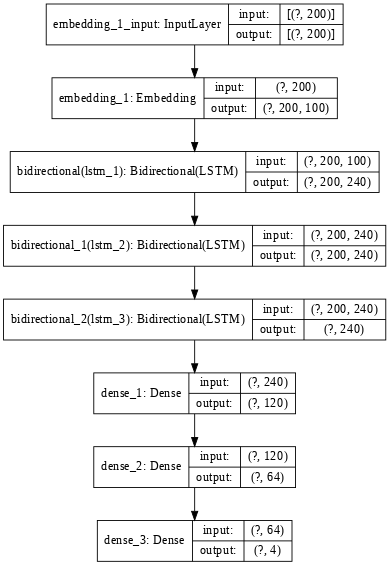
\includegraphics[width=8cm]{figures/reports/lstm_deep_graph.png}
\fcmfcaption{Graf przedstawiający budowę głębokiej architektury LSTM.}\label{rys:lstm_deep_graph}
\end{figure}

Kolejną modyfikacją było dodanie kolejnych warstw sieci gęstej. Wcześniej użytą jedną warstwę zawierającą 4 neurony wyjściowe rozszerzono o kolejne dwie warstwy gęste. Pierwsza z nich zawiera 120 neuronów a druga zawiera 64 neurony. Szczegóły tej budowy przedstawiono na rysunku \ref{rys:lstm_deep_table}, który przestawia tabelę prezentującą szczegóły budowy głębokiej architektury LSTM. Do dodanych warstw użyto innej funkcji aktywacji jaką jest jednostronnie obcięta funkcja liniowa (ang. \textit{ReLU}), która stała się standardem do użycia w wewnętrznych warstwach gęstej sieci neuronowej \cite{xu2015empirical}. W ostatniej warstwie także zamieniono funkcję aktywacji na funkcję \textit{softmax}, która lepiej nadaje się do klasyfikacji wieloklasowej.

\begin{figure}[t]
\centering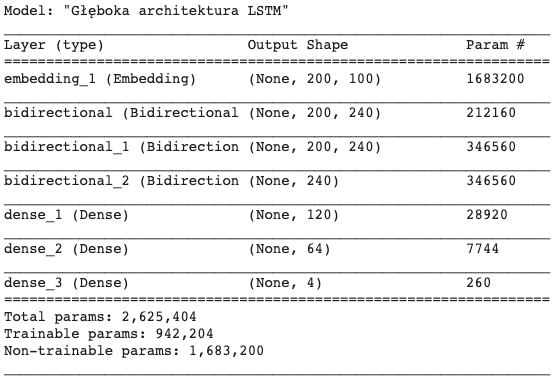
\includegraphics[width=10cm]{figures/reports/lstm_deep_table.png}
\fcmfcaption{Tabela przedstawiająca szczegóły budowy głębokiej architektury LSTM.}\label{rys:lstm_deep_table}
\end{figure}

Porównując dokonane rozszerzenia modelu z jedną warstwą LSTM, oraz wykonując opisane modyfikacje warstw zwiększyła się złożoność modelu. Prostym sposobem na porównanie modeli jest sprawdzenie liczby parametrów, które definiują zachowanie sztucznych neuronów, inaczej nazywane wagami neuronu. W tabeli \ref{tab:tabela_modele} przedstawione są liczby parametrów podzielonych na dwie grupy. Parametry trenowalne modelu to są wagi, które ulegają modyfikacji, liczba tych parametrów zwiększyła się około dziewięciokrotnie co ilustruję skalę zmian. Parametry stałe to są wagi użyte do generacji gęstych reprezentacji wektorowych, które były zamrożone na czas nauki modeli.  

\begin{table}[t]
\fcmtcaption{Tabela porównująca szczegóły budowy poszczególnych model.}\label{tab:tabela_modele}
\centering\footnotesize%
\begin{tabular}{c c c c}
\toprule
model & parametry trenowalne & parametry stałe & SUMA \\
\midrule
Jednowarstwowy LSTM   & 106,564 & 1,683,200 & 1,789,764 \\
Głęboki LSTM   & 942,204 & 1,683,200 & 2,625,404 \\
BERT todo   & xx & xx & xxx \\
\bottomrule
\end{tabular}
\end{table}

% \section{Głęboka architektura BERT}

% TODO \cite{devlin2018bert} BERT